% This is samplepaper.tex, a sample chapter demonstrating the
% LLNCS macro package for Springer Computer Science proceedings;
% Version 2.20 of 2017/10/04
%
%\documentclass[runningheads]{llncs}
\documentclass{llncs}
\pagestyle{plain}
%
\usepackage{graphicx}
\usepackage{caption}
\usepackage[l3]{csvsimple}
\usepackage{xcolor}
\usepackage{wrapfig}
\usepackage{subfig}
% Used for displaying a sample figure. If possible, figure files should
% be included in EPS format.


\graphicspath{ {./images/} }
\setcounter{secnumdepth}{3}
\setcounter{tocdepth}{5}

\pagenumbering{arabic}
\begin{document}
\begin{titlepage}
\title{

\includegraphics[width=1.75in]{images/UP_Logo.png} \\
\vspace{20pt}
\textbf{\huge Plan Merging Project}\\
}

\author{
\textit{\Large Project Report}\\
\vspace{20pt}
\textit{\large by}\\
\vspace{10pt}
\Large Anton Rabe\\
Aaron Bishop\\
Louis Donath\\
\vspace{20pt}
Under the supervision of\\
Etienne Tignon
\vspace{3cm}
}

\institute{\Large INSTITUTE OF COMPUTER SCIENCE\\ 
University of Potsdam\\
\vspace{1.5cm}
\large March 9th, 2022}
\end{titlepage}

\let\oldaddcontentsline\addcontentsline
\def\addcontentsline#1#2#3{}
\maketitle
\def\addcontentsline#1#2#3{\oldaddcontentsline{#1}{#2}{#3}}

\tableofcontents
\newpage
\begin{abstract}
When solving the plan merging problem, adding the constraint that only positions on the original paths can be used leads to only three options for modifying an agents plan: waiting, moving back and forth, and switching to another path. the latter, although not generally applicable to any warehouse situation, proves to be a powerful tool to resolve collisions and reduce the size of the input in a simple domain. In general plan switching and waiting can be applied sequentially to solve any instance and drastically reducing time complexity (divide and conquer). Furthermore, for both plan switching and waiting, incremental solving with repeated optimization is significantly faster than one-shot methods. On large instances where collisions often follow certain patterns it is also feasible to resolve vertex collisions using a deterministic one-model approach. This often proves more efficient than the incremental approach but is harder to implement and test consistently. Different approaches for plan switching and waiting can be combined in larger sequential algorithms that can be modified to fit certain instances.
%\keywords{First keyword  \and Second keyword \and Another keyword.}
\end{abstract}
\setcounter{page}{1}
\section{Introduction}
At least since the advent of online shopping, large quantities of products have to be managed in warehouses around the world. However, thanks to today's technical innovations, it is not necessary to do this by hand. At large shipping companies like Amazon, robots automatically deliver the required products from the shelf's to the packing stations where they are needed\cite{amazon}.\\
Therefore finding and optimizing paths of agents in simple environments is an important theoretical problem.
In this project, we try to provide a solution to a simple version of the plan merging problem using Answer Set Programming (ASP) in clingo \cite{clingo}. For a given warehouse scenario where robots are moving in a discrete labyrinth on initial individual plans we want to calculate a final plan that is guaranteed not to lead to any collisions or robots being blocked from their goals.
The input, we worked with, consists of a wharehouse represented by a set of cells and a set of robots that all have a plan represented by a sequence of moves. Our goal is to develop a merging algorithms that modifies the plans in such a way that all robots can simultaneously complete their tasks without colliding while still moving in a similar way as planned.  \\
After going over a specific description of the problem and what exactly defines good plan switching in our interpretation we will present several approaches to solve this problem and discuss their advantages and disadvantages based on their performance on human made benchmark instances. Finally, we will compare our approach with the results of the other groups in terms of optimality and time performance. \\

\subsection{Asprilo}
To illustrate the problem instances we used the Asprilo \cite{asprilo} framework. It offers different domains to simulate a warehouse on different levels of complexity. The A domain includes the ordering of specific amount of products from shelf's containing this product. In the B domain the amount is no longer taken into account. In this project we worked on the simplified M domain. 
\begin{wrapfigure}{r}{0.4\textwidth}
\centering
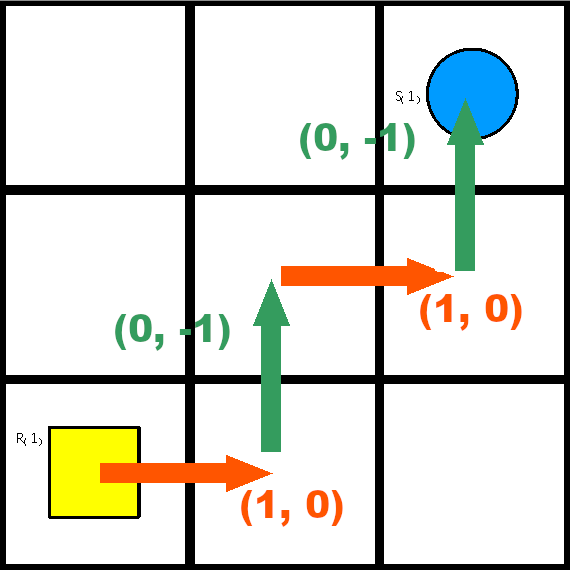
\includegraphics[width=.3\textwidth]{images/example_plan.PNG}
\caption{Example for the Plan of a Robot. The yellow square represents the robot and the blue circle represents the shelf it has to reach. The four moves of the robot are represented by the arrows.} \label{fig1}
\vspace{-20pt}
\end{wrapfigure}
Here the  goal is that each robot gets from its starting position to a shelf without a collision.\\
To work on the problem of multi agent path finding, Asprilo comes with some very useful tools. 
The visualizer
allows to convert a set of facts (like the position of each robot in each timestep) into a visual representation (the robots moving around). It also provides an instance generator that allows to create problem instances on a visual level, which are then converted into facts. \\
To implement our encodings we use clingo It allowed us to crate a search space, in which lots of possible scenarios were explored. For example, in one approach, we considered for each robot at each position, that it could be waiting.\\
\subsection{The idea of plan merging}
A possible solution to the problem of plan merging would be to simply use multi agent path finding to generate the plans in such a way that the robots reach their destination as quickly as possible, while avoiding collisions. If all possible plans were considered for all robots, this solution would guarantee optimality. The big disadvantage of such a method is that the runtime would be astronomical, since all combinations of all possible plans would have to be considered. \\
By only modifying the initial plans we can save time and stick more closely to the input which is being expected from a plan merging algorithm.
Instead of generating new plans from scratch plan merging should aim to resolve collisions locally and leave the overall shape of the original plan intact i.e. not to deviate from original plans to much.
%In order to solve the problem efficiently, while still maintaining an acceptable runtime, plan merging comes into place. Instead of trying out all possible plans, we start with a concrete plan for each robot. In this way, we can check step by step which problems arise and solve them.\\%
Still it is open to interpretation what deviation from the original plan actually means. 

The methods presented below are designed to meet a very strict interpretation of plan merging i.e. that only cells that lie on the original plans can be used in the final plan. Thus this approach is applicable in situations with little knowledge about the environment e.g. the position of walls.
By reusing information from the original plans the complexity of our algorithm should be significantly smaller than from scratch path finding. 
\newpage

When focusing only on cells that occur in original plans three different operations can be used to modify the original plan of a robot: 
\begin{itemize}
\item waiting at a position for a number of timesteps
\item moving back and forth on a plan
\item reassigning the goals for robots with overlapping plans i.e. branching of and following another robots plan when possible. 
\end{itemize}
Especially the latter is highly questionable because it means that even though we are only using sections from original plans to reconstruct new final plans the plan of an original robot may change drastically often even to the point where robots arrive at different goals. It is important that the assumption that goal assignment is arbitrary is generally not true in more complex domains i.g. when robots deliver goods. For this project we decided to allow plan switching and reassigning goals.\\
In general this plan switching step can be done as preprocessing reducing the size of the instance 




\newpage

\section{Problem description}
All instances are represented by a set of nodes or cells with coordinates. In general the Nodes can be populated with robots, shelf's and picking stations. Since we are working in the M domain, the picking stations are not a part of our problem description.
In this domain a complete instance consists of a set of robots and a set of shelf's, that are placed on the nodes. The goal of each Robot is to reach a certain shelf. Therefore each robot has an initial plan how to reach its destination shelf. The plans consist of a sequence of single moves. For example, the plan for the robot in Figure 1 is given by the sequence [(1,0), (0,-1), (1,0), (0,-1)]\\
Only moves between neighbouring nodes are possible. Diagonal movement is not allowed.
In an instance with multiple robots, the initial plans may overlap and cause collisions.\\
We refer to the case where two robots move to the same node at the same time as a vertex collision. The scenario of two robots swapping places so that at the next timestep both are at the previous position of the other robot is called edge collision.\\
Fig.2 shows examples of these two simple collision cases.
In addition to the points discussed in 1.2. the main task of the plan merging algorithm that we have developed in this project, is to find a way to redesign the plans of the robots in such a way, that no more collisions occur.

\begin{figure}[!h]
  \centering
  \subfloat[][]{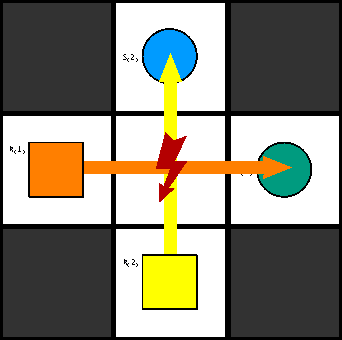
\includegraphics[width=.4\textwidth]{images/collisions/Vertex_collision.png}}\quad
  \subfloat[][]{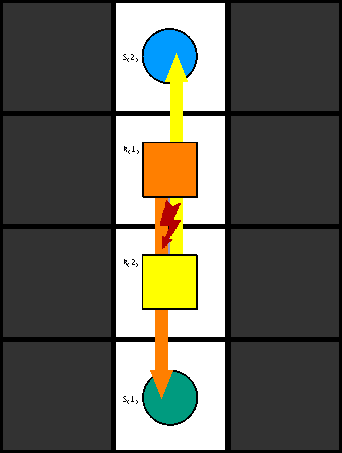
\includegraphics[width=.4\textwidth]{images/collisions/Edge_collision.png}}\\
  \caption{The two types of collisions that need to be prevented by applying plan merging: vertex collision (a) and edge collision (b).}
  \label{fig2}
\end{figure}

\newpage

\section{Plan Merging Approaches}

\subsection{Encoding the instance}
The position C of a robot R at a timestep T can be inferred from moves on the original plan and starting positions in a recursive manner using:
\begin{verbatim}
position(R,(X+DX,Y+DY),T+1) :- move(R,(DX,DY),T), position(R,(X,Y),T).  
 \end{verbatim}
From this several features of the original plan can be extracted including intersections between two paths, the last timestep of a plan corresponding to the goal and the length of the longest path which we will refer to as the horizon:
\begin{verbatim}
intersect(R,R',C,T,T') :- position(R,C,T), position(R',C,T'), R!=R'.
last_pos(R,C,T) :- position(R,C,T), not position(R,_,T+1).
horizon(T_MAX) :- T_MAX == #max{T : position(R,C,T)}.
\end{verbatim}
Collisions in the original plan are defined by 
\begin{verbatim}
vertex_collision(R,R',C,T) :- position(R,C,T), position(R',C,T), 
                              R!=R'.
edge_collision(R,R',T+1) :- position(R,C,T), position(R,C',T+1),   
                            position(R',C',T), position(R',C,T+1), 
                            R!=R'.
\end{verbatim}
Based on this information about the original plan we can deduct positions for waiting and switching. The way these positions are assigned is for the time performance of the final approach.

\subsection{Plan Switching}
Assuming only cells from original plans can be used in final plans and the direction of movement is fixed, many problems can only be solved using plan switching i.e. allowing robots to follow another robots plan following an intersection of two plans. 
This can effectively resolve edge collisions and edge collision-like vertex collisions (fake edge collisions) i.e. collisions between robots that move in opposite directions on the same cells.
Such collisions are represented by:
\begin{verbatim}
edge_collision(R,R',T+1) :- position(R,C,T), position(R,C',T+1),
                            position(R',C',T), position(R',C,T+1),
                            R!=R', C!=C'.
fake_edge_collision(R,R',T) :- position(R,C,T), position(R,C',T+1),
                               position(R',C',T-1), position(R',C,T),
                               R!=R', C!=C'.
\end{verbatim}
In addition to resolving edge collisions plan switching can also be used to drastically reduce the size of the instance.
Fig.3 shows two simple instances of original plans before and after plan switching. (a) is an example for a case that can be solved using waiting but also has a much shorter solution (c) when allowing plan switching. This instance contains an edge collision between robots R(2) and R(1) and edge-collision-like vertex collisions (fake edge collision) between R(1) and R(3) and R(2) and R(3).
The total number of steps in the original plans is 19 with longest path at 7 time steps. Using only waiting the shortest final plan that doesn't contain any collisions will have a horizon of 9 containing 21 steps. After plan switching the horizon is 6 and the final plan contains 11 steps. Thus for solving (a) plan switching is not needed but leads to a shorter more elegant solution (b).
On the other hand plan switching is necessary to remove the central edge collision in (c) assuming leaving the original plan is not possible.\\
\begin{figure}[!h]
  \centering
  \subfloat[][]{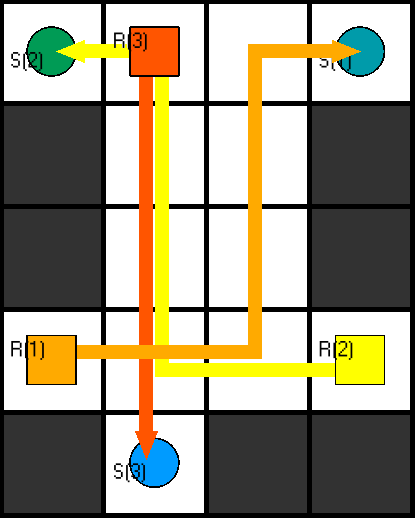
\includegraphics[width=.4\textwidth]{images/bm_plans/bm16_plans.png}}\quad
  \subfloat[][]{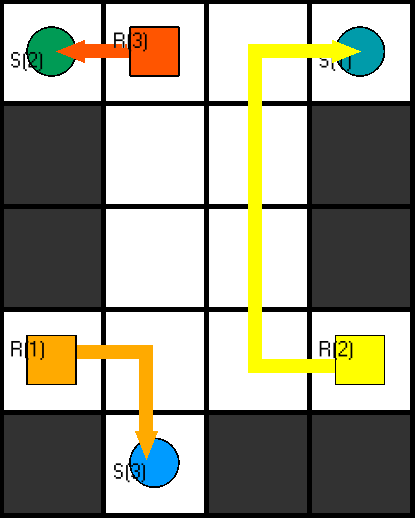
\includegraphics[width=.4\textwidth]{images/bm_plans/bm16_plans_switched.png}}\\
  \subfloat[][]{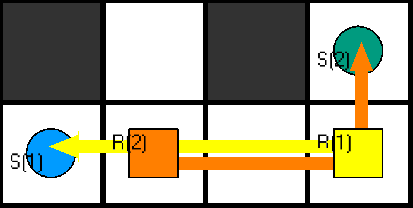
\includegraphics[width=.4\textwidth]{images/bm_plans/bm15_plans.png}}\quad
  \subfloat[][]{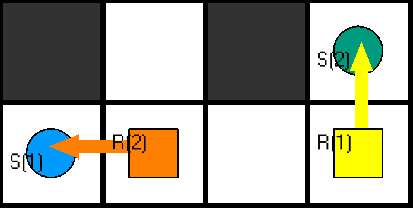
\includegraphics[width=.4\textwidth]{images/bm_plans/bm15_plans_switched.png}}
  \caption{Two instances (a) and (c) that can be solved using plan switching and the corresponding final paths (b) and (d).}
  \label{fig2}
\end{figure}
\\
A special case of vertex collision that can occur between robots moving in the same direction is also best resolved using plan switching.
If a robot is overtaking another robot that has reached its goal we can simply reassign the plan of the later robot to the robot that is already finished and make the later robot wait at the goal that lies on its path.
We refer to these cases as overtake collisions. They can be inferred from original positions using:
\begin{verbatim}
overtake_collision(R,R',T,T') :- last_position(R,C,T),
                                 position(R',C,T'), 
                                 R!=R', T'>T.
\end{verbatim}
Finally we represent a plan switch performed by a robot R occuring at time step T as a switch statement that contains the switching robot, the original robot that was moving on the new plan and the two time steps of the intersection where the switch occurs, i.e. the time step at which to leave the old path and continue on the new path. To allow robots following another robots paths position\_ statements must store information about the current identity of the robot R', i.e. which plan it is following, and the time step N on that plan. All robots start with R'=R and N=T=0. These parameters change during switching.
\begin{verbatim}
position_(R,C',T+1,R',N+1) :- position(R',C',N+1), 
                              position_(R,C,T,R',N), 
                              not switch(R',_,N,_).
position_(R,C',T+1,R'',D+1) :- position(R'',C',D+1),                   
                               position_(R,C,T,R',N),
                               switch(R',R'',N,D).
\end{verbatim}

Allowing all robots to switch at any intersection proves to be very hard to solve on instances with many intersections. To handle the increase in time complexity we use incremental solving in python.

\subsubsection{Incremental Plan Switching}

A central idea that is common to most final approaches presented here is to use ASP repeatedly in a recursive manner at each step optimizing a heuristic to find a fixed point that is guaranteed to resemble a consistent solution.\\
The ideas below are simplifications that limit the amount of possible models and help to reduce computation time of a single incremental step.
First we can reduce the amount of robots that can switch plans by only allowing those robots that are involved in an edge-collision or fake edge-collision to switch. Additionally instead of treating plan switching as one robot branching off, it can be implemented as pairwise switching between two robots.
\begin{verbatim}
{switch(R,R')} :- collision(R,R',T).
switch(R',R) :- switch(R,R').
\end{verbatim}
Additionally, we can fix the switching positions to the earliest intersect with the other robot. This will lead to the greatest decrease in path-length and will help quickly reduce the size of the instance.
\begin{verbatim}
switch(R,R',T,T'):- switch(R,R'), earliest_intersect(R,R',C,T,T').
\end{verbatim}
In the next iteration earliest\_intersect statements must be updated for resulting new plans. The best results regarding the overall time performance were achieved by recursively calculating optimal pairwise switching operations not allowing chains of multiple switches per robot using the following constraint.
\begin{verbatim}
:- switch(R,R'), switch(R,R''), R'!=R''.
\end{verbatim}

It is crucial to implement optimization in clingo \cite{clingo} in a way that guarantees that the iterative approach converges on the global minimum of zero edge collisions i.e. that the fixed point of incremental recursive solving with optimization always represents a valid solution.
Since each plan switching operation removes steps from individual plans, it is safe to minimize the total number of position\_ statements:
\begin{verbatim}
#minimize {1@4,T,R : position_(R,C,T)}.
\end{verbatim}
If a solution still contains edge collisions it will never have a minimal number of position\_ statements as the removal of an edge collision always results in the removal of at least two position\_ statements.
Furthermore the horizon parameter of the final plan can be minimized resulting in a drastic improvement in time performance:
\begin{verbatim}
horizon_(T_MAX) :- T_MAX == #max{T : position_(R,C,T,X,Y)}.
#minimize{T@5 : horizon_(T)}.
\end{verbatim}
Because an edge collision represents two robots moving in opposite directions on the same cells, a plan switching operation will always lead to the robots arriving at a goal at an earlier timestep. Thus the horizon can never grow and a solution with minimal edge collisions will also have minimal horizon. Thus a fixed point of horizon and number of collisions will always represent a solution with minimal edge-collision-like collisions.
Furthermore, by minimizing the total number of position\_ statements in the final plan the algorithm is guaranteed to avoid converging on local minima regarding the number of collisions as it prioritizes removing known collisions to reduce the number of steps.

\subsubsection{Preventive Plan Switching}
To guarantee that no new edge collisions are generated when applying the waiting algorithm it is not sufficient to remove edge collisions in the final plan. Fig.4 is an example for an instance that doesn't contain any edge collisions but would lead to a new edge collision if robot 2 is delayed because of waiting. \\
We need to extend the condition for pairwise switching to all pairs of robots that move in opposite directions on the same cells at any timestep i.e. all pairs of robots that could share an edge collision if they wait for the right amount of timesteps.
\begin{verbatim}
edge_collision_possible(R,R',T) :- intersect(R,R',C,T,T'), 
                                   intersect(R,R',C',T+1,T'-1).
\end{verbatim}
By minimizing all possible edge collisions we obtain paths where all intersections represent crossing paths or robots moving in the same direction. Applying plan switching with this condition for switching prevents edge collisions that could occur when waiting is applied.
The resulting instance often has shorter paths than the result of \emph{Simple Incremental Plan Switching} and can be much easier to solve using waiting.
However, this is also a much harder plan switching problem because the number of possible switching operations and thus the number of possible models is usually higher which leads to a massive decrease in time performance. Additionally, we can no longer include the horizon parameter in the optimization as single paths can become longer. Longer running times can be circumvented by only applying \emph{Preventive Plan Switching} recursively to the result of \emph{Simple Plan Switching} which is usually already a much smaller instance.

\subsection{Waiting}
Waiting for a number of time steps at a certain position in the original plan is a simple method to resolve vertex collisions between robots that are moving in the same direction. After \emph{Preventive Plan Switching} has been applied the modified instance will only contain collisions between robots moving in the same direction that can be removed using waiting. 
Fig.4 shows a typical instance that is best solved using waiting. All collisions occur between robots that move in the same direction and there are no overtake collisions or edge collision like intersections.
After preprocessing, all remaining vertex collisions follow this pattern. The main difficulty for the waiting algorithm is to avoid creating new collisions by making one robot arrive later at an intersection or making a robot run into a waiting robot.
\begin{figure}
    \centering
    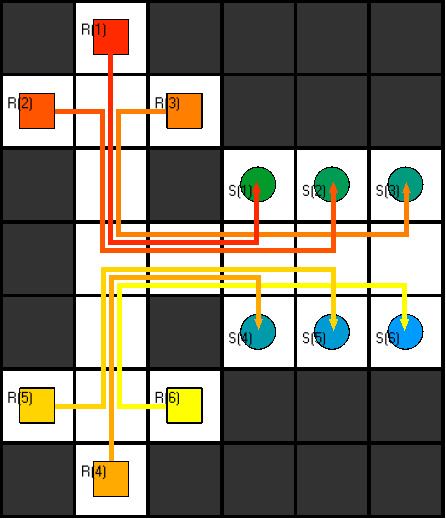
\includegraphics[scale=0.5]{images/bm_plans/bm_8_plans.png}
    \caption{A simple warehouse situation were robots need to form a queue using waiting.}
    \label{fig:my_label}
\end{figure}
A robot R waiting at time step T of its original plan can be represented by a wait statement. After calculating or choosing waiting times position\_ statements can be generated like this
\begin{verbatim}
position_(R,C,T+1,N+1) :- position_(R,C,T,N), wait(R,_,T).
position_(R,C',T+1,N) :- position(R,C',T-N+1), not wait(R,_,T),     
                         position_(R,C,T,N).
\end{verbatim}
To properly calculate the next step after multiple waits we need to store the number of waits as N. The next cell C' in the original plan for a given position\_ is then given by position(R,C',T-N+1).\\
Simple implementations of waiting include layer based methods (\emph{Layer Approach}) where waiting positions are calculated one conflict at a time incrementally updating the plans. Each layer will then contain a full plan after one vertex collision is resolved. This is quite costly in time and space. Furthermore, this approach depends on a sound metric for assigning the priority of each robot at each collision.
Later we will see that we can actually calculate waiting positions from intersects and collisions on the original plans in a deterministic way not updating the paths and thus achieving much better time performance.\\
Another approach is allowing robots to wait at any position and treating the problem as a constraint satisfaction problem (CSP) using choice rules and optimization. This is extremely slow on benchmarks with long paths even if possible waiting positions are limited to one time step before first intersections of two robots. Again we can reduce time complexity by breaking down the problem into incremental steps and recursively optimizing a heuristic.

\subsubsection{Incremental Waiting}
Following the preprocessing of both \emph{Simple and Preventive Plan Switching}, there should not be any immediate edge collisions as well as potential edge collisions caused by waiting left in the plans. Unfortunately, plan switching does not accommodate the removal of vertex collisions in the slightest. Therefore, the robots have to be able to wait at certain time steps before proceeding with their plans in order to resolve those vertex collisions. Due to the optimality of the solution but quick blow up in time that comes with using the \emph{Naive Choice Rule Waiting}, which allows robots to wait a limited number of times on every single position, it is natural to make efforts of improvement whilst adhering to the same concept of non-deterministic waiting using choice rules.
One way of reducing the size of the search space is by dividing the problem into smaller chunks that can be more manageable for the solver. For the \emph{Incremental Waiting} the problem gets broken down to a situation where robots that are involved in a vertex collision have the ability to wait once or not at all.
From there, we want to find a model that minimizes the number of vertex collisions without waiting unnecessarily or causing any new edge collisions.
By repeating this process incrementally, the number of vertex collisions will decrease until convergence.

The head of the encoding consists of rules that find the bare minimum of possible waiting times for each robot.
\begin{verbatim}
% find times for waitable positions
has_vc(R,R') :- position(R,C,T), position(R',C,T), R!=R'.
waitable(R,T) :- has_vc(R,R'), position(R,C,T+1), 
                 position(R',C,T'), R!=R'.
waitable(R,T) :- waitable(R',T), position(R,C,T+1),
                 position(R',C,T'), R!=R'.
not_earliest_waitable(R,T) :- waitable(R,T), waitable(R,T'), T>T'.
earliest_waitable(R,T) :- not not_earliest_waitable(R,T), 
                          waitable(R,T).
\end{verbatim}

First, the pairs of robots involved in the same vertex collision get gathered in the \emph{has\_vc/2} predicate. Only robots involved in vertex collisions are able to find potential waiting times from there.
These waiting times are true when a robot is exactly one step before intersecting with the path of a robot he will later collide with. The second rule that can make atoms of the \emph{waitable/2} predicate true allows robots that intersect with other possibly waiting robots to wait as well. Otherwise, a robot in a queue will crash into his front neighbor if he suddenly chooses to stop.
Finally, only the earliest occuring waitable time is actually being used in the following choice rule.

\begin{verbatim}
% either wait at one waitable timestep or don't
{wait(R,T) : earliest_waitable(R,T)}1 :- isRobot(R).
\end{verbatim}

This choice rule produces a large number of potential models where all robots that have an earliest waitable time are either waiting at that time or not. Therefore, the size of the search space is highly dependent on the number of robots involved in vertex collisions as well as the number of robots that intersect with them. And due to the binary decision that is made for each robot, the number of potential models will equal $2^n$, with $n = $ number of robots, in the worst case scenario.

\begin{verbatim}
% reconstruct positions
% before wait
position_(R,C,T) :- wait(R,T_WAIT), T<=T_WAIT, position(R,C,T).
% after wait
position_(R,C,T) :- wait(R,T_WAIT), T>T_WAIT, position(R,C,T-1).
% keep positions if no wait
wait(R) :- wait(R,T).
position_(R,C,T) :- not wait(R), position(R,C,T).
\end{verbatim}

Here, the wait instruction will get incorporated into the new plans by reconstructing them within the \emph{position\_/3} predicate which is used for the output later.

\begin{verbatim}
% find new vertex collisions
horizon(R,T_MAX-1) :- T_MAX == #count{T : position_(R,C,T)},
                      isRobot(R).
vc_cost(R,T,(T_MAX-T)*(T_MAX-T)) :- position_(R,C,T), 
                                    position_(R',C,T),
                                    R!=R', horizon(R,T_MAX).
\end{verbatim}

The resulting vertex collisions are then counted in the \emph{vc\_cost/3} predicate. But instead of merely using the number of vertex collisions for the following minimization, a cost is formulated.\\ This cost is defined by $cost = (T_{MAX} - T_{VC})^2$, where $T_{MAX}$ is the maximum time step of a robot and $T_{VC}$ is the time step of a vertex collision. The goal of this cost is to prefer later collisions strongly over earlier ones. So, in the case where it is not sufficient to minimize the number of vertex collisions by letting robots wait only once, the program will at least try to delay these collisions.
This helps to direct the solution towards the global minimum as opposed to falling into a local minimum.

\begin{verbatim}
% remove new edge collision
:- position_(R,C,T), position_(R,C',T+1), position_(R',C',T),
                     position_(R',C,T+1), R!=R', C!=C'.
% remove new fake edge collision
:- position_(R,C,T), position_(R,C',T+2), position_(R',C',T),
                     position_(R',C,T+2), R!=R', C!=C'.
% remove new vertex collisions with arrived robots
destination(R,C,T) :- position(R,C,T), not position(R,_,T+1),
                      isRobot(R).
:- position_(R,C,T), destination(R',C,T_DEST), T>T_DEST, R!=R'.
\end{verbatim}

Integrity constraints are always a part of a constraint satisfaction problem and are needed here to quickly rule out any models that cause new edge or overtake collisions to appear since they can never be solved by waiting.

\begin{verbatim}
% minimize number of waits
#minimize {1@1,R : wait(R,T)}.
% minimize number of vertex_collisions or at least delay them
#minimize {C@2,R,T : vc_cost(R,T,C)}.
\end{verbatim}

Finally, in the optimization section, the costs for the new vertex collisions get minimized with higher priority before minimizing the number of wait instructions to avoid unnecessary waiting.
And as previously mentioned, this entire process gets repeatedly invoked until convergence is reached.

\subsubsection{Deterministic Waiting}
After plan switching has been applied all collisions left in the preprocessed plan will be vertex collisions between robots that are either crossing each others paths or moving in the same direction.
Because this problem is highly systematic it is feasible to remove most if not all the remaining vertex collisions by inferring all final positions directly from features of the original plan in a single model. By nature this deterministic one-model approach is much faster on large instances than assigning waiting positions using choice rules as it does not have to deal with the combinatorial explosion of the number of models.
This approach for assigning the waiting positions came up at a later stage of the project and still has a lot of room for improvement especially in time performance.
Since the preprocessed plans do not contain any overtake collisions, The length of the remaining path is a valid metric for defining the priority of a robot when resolving a conflict. A robot with a shorter remaining path should always wait for a robot with a longer remaining path because reversing their order could create an overtake collision. Combined with choosing the robot with the larger ID, in case of a tie this leads to a deterministic formula for the priority of a robot at a collision.
By not making robots with longer paths wait we also avoid generating extremely long and thus not optimal final plans. 
We can represent the hierarchy of robots with simple higher/2 atoms indicating R' has priority over R.
\begin{verbatim}
higher(R,R'):- earliest_collision(R,R',C,T), 
               last_time(R,D), last_time(R',D'),
               D-T<D'-T.
higher(robot(A),robot(B)):- earliest_collision(robot(A),robot(B),C,T),
                            last_time(robot(A),D), last_time(robot(B),D')
                            D-T=D'-T, A<B.  
\end{verbatim}
We can now calculate the number of waits for a robot at a collision from the number of robots that take part in the same conflict but have higher priority.
This works fine on extremely systematic instances like Fig.4 but leads to trouble when robots that arrive later at the position of a collision run into waiting robots or if waiting delays a robot creating new collisions.
To calculate the accurate amount of waits the delay of robots that already have waited needs to be factored in. Thus we need to count the number of waits that a robot performed before a collision. 
\begin{verbatim}
waited_so_far(R,0,0):- isRobot(R).
waited_so_far(R,T+1,A):- waited_so_far(R,T,A), position(R,_,T+1),
                         not do_wait(R,_,T,_).
waited_so_far(R,T+1,A+B):- waited_so_far(R,T,A), position(R,_,T+1),
                           do_wait(R,C,T,B).
\end{verbatim}
do\_wait atoms represent the amount of waits that are assigned to a specific time step after the priority of the robot at a conflict has been computed.
To accurately derive the amount of waits we need to find the robot that has the next highest priority and factor in the amount of waits it has performed.
\begin{verbatim}
prio(R,C,T,A) :- earliest_collision(R,R'',C,T),  
        A == #count{1,R' : collision(R,R',C,T), higher(R,R')}.

new_r_ahead(R,C,T,A) :- earliest_collision(R,R'',C,T),
                A == #count{1,R' : earliest_collision(R,R',C,T), 
                higher(R,R')}.

wait_for(R,C,T,W'-P'+B'+P) :- earliest_collision(R,R',C,T), 
                              prio(R',C,T,P'), prio(R,C,T,P) , 
                              new_r_ahead(R',C,T,B'), 
                              waited_so_far(R',T-1,W'), P'<P.

not_wait_for(R,C,T,P) :- wait_for(R,C,T,P), wait_for(R,C,T,P'), P<P'.

do_wait(R,C,T-1,A-W) :- waited_so_far(R,T-1,W), 
                        wait_for(R,C,T,A), 
                        not not_wait_for(R,C,T,A), A-W>=0.
\end{verbatim}
To prevent robot collisions with waiting robots, robots that do not participate in a collision but get there soon after they need to wait as well if they are close enough to run into the last waiting robot. To prevent unnecessary waiting the number of waits can be calculated from earlier waiting operations and the distance in time steps to the collision. The later\_at\_collisions statement represents the case that a robot arrives at the position of a collision at T' after the timestep T of the collision.
\begin{verbatim}
do_wait(R,C,T-1,A-W) :- later_at_collision(R,R',C,T,T'), 
                        prio(R',C,T,P), not prio(_,C,T,P+1),
                        waited_so_far(R',T,A), waited_so_far(R,T-1,W).
\end{verbatim}
With these changes applied only  robots that do not share collisions or non mutual collision positions on their paths can have vertex collisions if the robot that arrives first at an intersection has waited before. The following statements help avoiding this. They are, however, very hard to ground on some instances. 
\begin{verbatim}
do_wait(R',C,T'-1,T+A-T'-A'+1) :- intersect(R,R',C,T,T'), 
                                  not later_at_collision(R',R,_,_,_), 
                                  not earliest_collision(R,R',_,_),
                                  waited_so_far(R,T,A),
                                  waited_so_far(R',T'-1,A'), 
                                  T<T', T+A>=T'+A'.

do_wait(R',C',T'+A'-1,X) :- intersect(R,R',C',T,T'), 
                            not later_at_collision(R',R,_,_,_), 
                            not earliest_collision(R,R',_,_), 
                            waited_so_far(R,T,A), 
                            waited_so_far(R',T'-1,A'), 
                            T<T',  T+A+1=T'+A', 
                            do_wait(R,C,T+A,X).

\end{verbatim}
Even without this extension, deterministic waiting often removes most vertex collisions from many instances. We refer to deterministic waiting without these rules as \emph{Minimal Deterministic Waiting} compared to \emph{Comprehensive Deterministic Waiting} including these two lines.
Because of the sequential nature of our approach there are a number of possible alternatives to this, for example trying minimal deterministic waiting and only running comprehensive waiting if minimal deterministic waiting could not find a consistent solution. Another possibility would be to remove remaining vertex collisions using incremental waiting as their number is often much lower after deterministic waiting.
In the next section we will outline how we can apply the different approaches sequentially to solve the plan merging problem and 

\subsection{Combined Approach}
In general waiting can be applied after plan switching as \emph{Preventive Plan Switching} prevents any new edge collisions from being generated by waiting robots. An instance with no more edge-collision-like intersects and overtake collisions can be solved using waiting without generating new collisions. To reduce running time we first apply \emph{Simple Plan Switching} followed by \emph{Preventive Plan Switching}. After this we can apply either \emph{Incremental Non-Deterministic Waiting} or \emph{Deterministic Waiting}. The exact order of operations can be modified leading to differences in time performance, optimality and consistency. For example in many cases \emph{Preventive Plan Switching} or \emph{Comprehensive Deterministic Waiting} is not necessary. One possibility to speed up the final algorithm would be to select the right components based on the instance. However, testing different metrics and heuristics to find the optimal composition of switching and waiting scripts exceeds the scope of this project.
A simple alternative is trying the minimal approach first and only executing comprehensive waiting and preventive switching if the first shot solution still contains collisions. This can actually be reasonable depending on the instance. 
Combining simple deterministic waiting with incremental non-deterministic might also be a valid alternative to comprehensive deterministic waiting. The different configurations of the sequential plan merging algorithm presented here must be evaluated with regard to time performance, optimality and consistency.
To realize recursive optimization, the sequential application of waiting, and enabling the testing of different configurations we implemented a python class that represents our sequential plan merging approach using the \emph{clingo API} \cite{api}.

\subsubsection{Implementation of the Merger Class}
In order to implement the combined approach whilst maintaining a clean, uncluttered and reusable code, we have created the \emph{Merger} class in \emph{Python}.\\
It features the following methods:
\begin{verbatim}
Interface Merger:

Model, AccumulatedStats : merge(str : benchmark, ...)

Model, AccumulatedStats : convertToPositions(Model : model, ...)
Model, AccumulatedStats : switchPlans(Model : model, bool : small, ...)
Model, AccumulatedStats : wait(Model : model, bool : deterministic, ...)
Model, AccumulatedStats : convertToAsprilo(Model : model, str : benchmark, ...)
Model, AccumulatedStats : checkValidity(Model : model, ...)
    
... more auxiliary methods

\end{verbatim}

The core of the \textbf{Merger} class is the main method \textbf{merge} which takes a path-like string pointing to a benchmark directory that includes an instance and the corresponding plans. The other arguments are optional and can be used to gain high-level control on the merging process e.g. choosing a plan merging approach, vizualizing the result, saving the resulting data, etc. Most importantly, it features an \textbf{bool : automatic} argument that will initiate an automatic benchmark-dependent approach-choosing algorithm.\\
As result, the \textbf{merge} method will return the solution of our sequential plan merging in form of an instance of the \textbf{Model} class as well as an instance of the \textbf{AccumulatedStats} class. Both of which have been created by our group.

The \textbf{Model} class contains a model of a \emph{clingo} solver in \emph{string} format as well as metadata about the model e.g. satisfiability, cost, statistics, etc.\\
The purpose of the \textbf{AccumulatedStats} class is to monitor statistics about all the intermediate results of a sequential algorithm. This includes, adding up the individual computation times for each step and yielding just one final computation time for the entire process.

Since the sequential approach comprises of multiple successive steps, the steps of converting the plans into \emph{position/3} predicates, switching between plans, adding wait instructions, converting back to an asprilo format and checking the validity are seperated into single methods that can be called individually.

Furthermore, plenty of auxiliary methods required for the core methods, presented above, are defined and implemented in the class too.



\section{Evaluation}
\subsection{Benchmarks}
Throughout the course of our project, we constantly have been testing our latest encodings on different benchmark instances to verify the integrity and quality of our plan merger. All of the benchmarks stored in our \emph{GitHub} repository \cite{project1} are tailored to test a specific feature of our encoding. For the first benchmarks this includes the isolation of vertex and edge collisions. As our work began to progress beyond these simple problems, we could venture towards more complex testing scenarios from multiple simultaneous collisions to novel consecutive collisions caused by the algorithm during the solving process. As soon as these types of very particular benchmarks were solvable for our merger, the problem of having a good time performance became a central criteria for evaluating our approach. Thereby, there was a lot of time spent on improving the time performance of our plan merging algorithms which is why there are some very large instances to be found in our repository. These types of benchmarks are intended really put the time complexity of a plan merging encoding to a test. Thus, some of our old and highly inefficient approaches e.g. \emph{Layer Approach} and \emph{Naive Choice Rule Waiting} are not able to solve these within acceptable time.
For this paper and the following sections, based on the size of the benchmarks inside our repository, we will define an ``unacceptable time'' as a total computation time above five minutes which will result in a lack of an entry inside a table.



\subsection{Benchmark Tool}
In means of aiding in the process of custom benchmark creation for all of the groups, we have developed the \emph{Benchmark Tool}\cite{project1} in \emph{Python}. It allows a user to create their own benchmarks, including the instance and plans, by interacting with an intuitive, quick and easy ``Graphical User Interface (GUI)''. Of course there are other ways of doing this, whether by writing the logical program of facts manually or using the asprilo vizualizer and its instance creation functionalities. But in practice, a lot of time had been saved using our tool because it is tailored towards our specific needs within this project. Mainly, this is due to the reasons that we are focusing solely on the M-domain and require the presence of predefined paths for each robot as input for the plan merger. Also, this tool will export and import a benchmark in the correct directory structure and naming convention according to our groups agreed benchmark format.


\subsection{Evaluation Setup}
The goal of the evaluation is to verify the quality of our various plan merging approaches by quantifying their results on all of our benchmarks to compare them with each other.
For this, all the groups taking part in the plan merging project have agreed to save the information of a result in a ``Java Script Object Notation (json)'' file of the given format:

\begin{verbatim}
"groupName" : "",
"solverName" : "",

"problemType" : None,
"objective" : None,
"objective_cost" : [],

"instance" : None,
	"statistics" : {
	"groundingTime" : 0.0,
	"solvingTime" : 0.0,
	"total" : 0.0,
	"atoms" : 0.0,
	"rules" : 0.0
},
"info" : "",
"model" : ""
\end{verbatim}

As shown above, this format contains information about the merging method and the benchmark instance that have been used. Most importantly, there are statistics about the total, grounding and solving time and the number of atoms and rules that were generated by \emph{clingo}\cite{clingo} to be found in the json format. These statistics are necessary to evaluate the performance of a solution.\\
The model which the merger outputted is attached as well in \emph{string} format and can be further analyzed to check the optimality of the solution by looking at different criterea, such as the horizon, the ``sum of all path lengths (SOAP)'' and some kind of metric to quantify the deviation to the original plans.
The latter is not useful for our merging approaches since we never allowed any robots to deviate from the original plans besides switching them and inserting waits. Obviously, before checking the optimality of a model we must ensure the validity or correctness of the solution, which is why we run the \emph{validity\_checker.lp}\cite{project1} at the end of the merging process. In this way, there will not be any false results that may contain residual collisions, erroneous movement of robots or the unfulfillment of orders at the horizon.\\
In our case, we are focusing a lot on the total computation time and the SOAP to compare results.
The total computation time will suffice as a time metric because it combines both the grounding and solving time. Atoms or rules are not beneficial to use for us since we chose a sequential plan merging approach which makes it hard to keep track of the actual amount of atoms and rules needed for the entire process. Simply summing the number of atoms and rules up is not adequate. But the amount of atoms and rules will also partially manifest itself inside the total computation time.
The SOAP is a good measure of verifying the optimality of a model when there is no plan deviation present.\\
Now, we can properly carry out a comparison between results by looking at these two metrics that we obtain by running a plan merger on a benchmark of choice.


\subsection{Results}
For the sake of comparability and reproducibility, all of our internal results have been computed on a machine with the following specifications:
\begin{verbatim}
System type:    x64-based PC
CPU:            Intel i5-6600K CPU @ 3.50GHz, 4 Cores
RAM:            16GB, DDR4
\end{verbatim}



This section will cover the analysis of the results of our best plan merging approaches on selected benchmarks that are interesting regarding the time performance. Then, we will use the metrics of the previous section to compare these approaches with each other and find the best approach for a given benchmark. This is necessary since the results are highly dependent on the benchmark that they are being run on. In the end we want to find a mapping of benchmarks to plan merging approaches that will automatically decide which approach to use by looking at some of the attributes of a benchmark.\\

\subsubsection{Error of the Results}
Without getting too technical into the statistics we want to at least take a quick look into the empirical standard deviation of the total computation times that we obtain in our results to see how large the error can be. This is necessary for the following comparison in order to tell if a result is better than another or if it simply lies within the error range and is actually equally good or potentially worse. To find the error of the results, we have computed one of our encodings (\emph{Comprehensive Deterministic Waiter}) on the same benchmark (\emph{Preprocessed Benchmark 25}) five hundred times and looked at all the resulting computation times. The result of the experiment shows that $std = 0.0046$ and $max - min = 0.0575$. It also shows that $97.4\%$ of the data lies within three standard deviations and $99.6\%$ within four standard deviations. Therefore, we define the error range within four standard deviations as ± 0.0184 or for simplicity ± 0.02.
This means that if two total computation times are being compared with a difference of less than 0.02 seconds, we can not deduce that one is better.


\subsubsection{Benchmark Selection}
For the purpose of this comparison, it makes sense to focus on the rather large benchmarks that we have made because the small ones will take a very short amount of time to solve on either of the two approaches. In addition, they do not make a lot of space for suboptimality due to the short path lengths of the robots, if we choose to use that as a metric.\\
Thus, we will pick the following benchmarks for the comparison:
\begin{itemize}
    \item \textbf{Benchmark 13:} 13\_time\_ performance
    \item \textbf{Benchmark 14:} 14\_big\_time\_performance
    \item \textbf{Benchmark 20:} 20\_big\_symmetric
    \item \textbf{Benchmark 22:} 22\_tons\_of\_vertex\_collisions
    \item \textbf{Benchmark 23:} 23\_half\_tons
    \item \textbf{Benchmark 25:} 25\_chaos
    \item \textbf{Benchmark 26:} 26\_diagonal\_chaos
\end{itemize}

These benchmarks are the largest in our collection and all focus on different aspects. Benchmark 22 for example is trivial for the plan switcher because all robots are heading through the same bottleneck. But it is a great challenge for our waiting encoding to solve due to the great number of robots and initial vertex collisions. On the other hand, Benchmark 14 and Benchmark 26 highly depend on the preprocessing step of plan switching to simplify the job for the waiting. Thus, a lot of computation time is lost on the plan switching.


\subsubsection{Approach Selection}
On the basis of many tests throughout our project, we have been trying out various approaches, as mentioned earlier, where we could quickly differentiate between viable options and less viable ones such as the \emph{Layer Approach} or the \emph{Naive Choice Rule Waiter} that caused the computation time to explode on bigger benchmarks.\\
Near the end of our project we have worked mostly on a \emph{Sequential} plan merging approach which lead us to have better performance. This took us even one step further to the \emph{interative fixed point solving} of the plan switching step and the waiting step.
Therefore, we will stick with only the \emph{Sequential} methods and will compare between:
\begin{itemize}
    \item \textbf{Simple + Preventive Plan Switching + Incremental Waiting}
    \item \textbf{Simple + Preventive Plan Switching + Deterministic Waiting}
\end{itemize}

But before proceeding, we must find a way to incorporate both of our different deterministic waiting encodings. Either \emph{Minimal Deterministic Waiting} or \emph{Comprehensive Deterministic Waiting} as well as \emph{Minimal Deterministic Waiting + Incremental Waiting} can be chosen for the deterministic waiting approach.\\
Let us compare the three methods on preprocessed plans which includes \emph{Simple Plan Switching} followed by \emph{Preventive Plan Switching} to pave the path of deterministic waiting.

\begin{table}[]
    \centering
    \csvautotabular{tables/det_small_iso.csv}
    %\hspace{1cm}
    \csvautotabular{tables/det_big_iso.csv}
    %\vspace{1cm}
    \csvautotabular{tables/det_small_inc_iso.csv}
    \vspace{1cm}
    \caption{Comparison of total computation times and residual conflicts between the minimal deterministic waiting and comprehensive deterministic waiting as well as minimal deterministic waiting plus incremental waiting. If ``conflicts'' is \emph{True}, there are still conflicts left and the result is not valid.}
    \label{tab:tab1}
\end{table}
\newpage
\begin{table}[]
    \centering
    \csvautotabular{tables/det_iso.csv}
    \vspace{1cm}
    \caption{This table compares the total computation times of the three different deterministic waiting strategies on large benchmarks. The ``X'' mark indicates that the strategy on that benchmark is the best and reaches out of the error interval. If there are multiple ``X'' markings for one benchmark, it means that these strategies lie inside the error interval and are equally good. These markings are only made for results that are exempt of conflicts.}
    \label{tab:tab1}
\end{table}

This comparison shows that the \emph{Minimal Deterministic Waiting} strategy is best for most benchmarks except for the two largest ones being Benchmark 25 and Benchmark 26. Thus, \emph{Comprehensive Deterministic Waiting} can be used on them instead. The \emph{Minimal Deterministic Waiting + Incremental Waiting} does not seem to be a strategy that is worthy of further persuit.
But for the following comparisons we will use the \emph{Comprehensive Deterministic Waiting} to ensure the validity at the cost of some additional total computation time.


%\newpage
\subsubsection{Attributes of a Benchmark}
To get closer to finding a mapping of benchmarks to approaches, we must look into the strengths and weaknesses of both plan merging approaches. One way of doing this is to take a deeper look into the attributes of a benchmark that causes a drastic change in either the total time or the SOAP in one of the two solutions.\\
But, let us first view the results of the two approaches on the selected benchmarks.\\

\begin{table}[]
    \centering
    \csvautotabular{tables/inc.csv}
    \hspace{1cm}
    \csvautotabular{tables/det.csv}
    \vspace{1cm}
    \caption{Comparison between the non-deterministic incremental approach and the determinstic approach using \emph{Comprehensive Deterministic Waiting} on prespecified benchmarks.\\
    \textbf{dSOAP} denotes the difference between the SOAP of the solution and the SOAP of the original plans. Thus, a negative dSOAP indicates the reduction of steps opposed to a positive dSOAP where steps had been added.}
    \label{tab:tab2}
\end{table}
\newpage
The most dramatic difference between results is clearly when one of the approaches is able to solve a benchmark within acceptable time while the other can not. In such a case, we must find the characteristic attributes of that particular benchmark and hopefully find a causal metric responsible for the failure.
This is the case for the incremental waiting approach on benchmark 22 due to the lack of an entry.


\begin{table}[]
    \centering
    \csvautotabular{tables/det-inc.csv}
    \vspace{1cm}
    \caption{This Table shows the difference between the deterministic and incremental approach mentioned above. When total(det) - total(inc) is less than zero, the deterministic approach was faster.\\
    When dSOAP(det) - dSOAP(inc) is less than \emph{0.0}, the deterministic approach was more optimal.}
    \label{tab:tab3}
\end{table}

After looking on the table above, we can see a significant difference in time for Benchmark 23 despite of the same optimality. Benchmark 25 is the only other Benchmark that seems to show another significant difference. But this is a difference in the optimality and less in the total time.

The next step is to take a deeper look into some benchmark attributes. But instead of looking at the raw benchmarks, it is necessary to look into the attributes of the preprocessed benchmarks. This means that the plan switching process has already been completed. The reason for that is that the main difference between our two approaches is the waiting and not the plan switching step and the waiting step works with the preprocessed steps. Besides, the interesting Benchmarks 22, 23 and 25 are all benchmarks that are hard problems regarding the waiting. Thus, we will look into them.

\begin{table}[]
    \centering
    \csvautotabular{tables/bm_metrics_after_ps_small_mini.csv}
    \vspace{1cm}
    \caption{A table with important attributes of all of our preprocessed benchmarks.\\
    \textbf{n robots} denotes the total number of robots present in the instance.\\
    \textbf{n pos} equals the SOAP.\\
    \textbf{horizon} equals to the length of the longest path.\\
    \textbf{n vcs} denotes the number of vertex collisions.\\
    \textbf{n robots had vcs} denotes number of robots who are involved in vertex collisions.\\
    \textbf{n ecs} denotes the number of edge collisions.\\
    \textbf{n robots had ecs} denotes number of robots who are involved in edge collisions.\\
    }
    \label{tab:tab1}
\end{table}
\newpage
We observe very high values for robots being involved in vertex collisions for Benchmark 22 and 23. This makes sense because the \emph{Non-deterministic Incremental Waiting} allows only robots to wait which are involved in a vertex collision. Benchmark 25 has a value of 9 which is not too high compared to easier to solve benchmarks like Benchmark 14, 19, 20, 21, 24 and 26. But in Benchmark 25, the number of total positions is the highest among those. All other attributes do not seem to be correlated with the cause of the significant differences in both time and optimality.
From this, we can deduce that there is a strong correlation between the total computation time of the \emph{Incremental Waiter} and the number of robots involved in a robot. Therefore, it makes sense to use it as a metric to make a decision on which approach we should choose for the solving. Besides this, the number of all positions which is nothing else than the SOAP can be used as a metric as well, since this seems to have an influence on the running time and length of the final plans. Obviously, it does not make sense for the SOAP to determine the optimality of a model but a high initial SOAP yields more local minima of optimality that the \emph{Incremental Waiting} may fall into.

\subsection{Between Group Comparison}
After testing our different approaches on large benchmarks we also compared our final plan merging solution to the other groups that took part in the Intelligent Logistics Project in order to fully assess the quality of our solution. In this semester, four groups have participated in the project.
\begin{itemize}
    \item \textbf{Group 1:} A. Simon, F. Franz\cite{project2}
    \item \textbf{Group 2:} A. Bishop, A. Rabe, L. Donath (our group)\cite{project1}
    \item \textbf{Group 3:} A. Romer\cite{project3}
    \item \textbf{Group 4:} D. Schreitter Ritter von Schwarzenfeld, J. Westphal and N. Bröcker\cite{project4}
\end{itemize}

For the coordination between the groups, we have cooperated by providing a package \emph{FinalMergingPackage}\cite{project1} that includes only our final plan merger together with our benchmarks packed into single .lp files. On the surface there is a python script that provides the ``merge'' function which takes an absolute path to a benchmark file and outputs the result into a json file into a given directory. This allows a user to easily import and use our plan merger on their own machine and collect data.

After collecting the data of all groups, we represent the results for the comparison in the following table. All the results have been computed on a machine with the following specifications:
\begin{verbatim}
System type:    x64-based PC
CPU:            Intel i7-8550u CPU @ 4.00GHz, 4 Cores
RAM:            8GB, DDR4
\end{verbatim}
\newpage
\begin{figure}
    \centering
    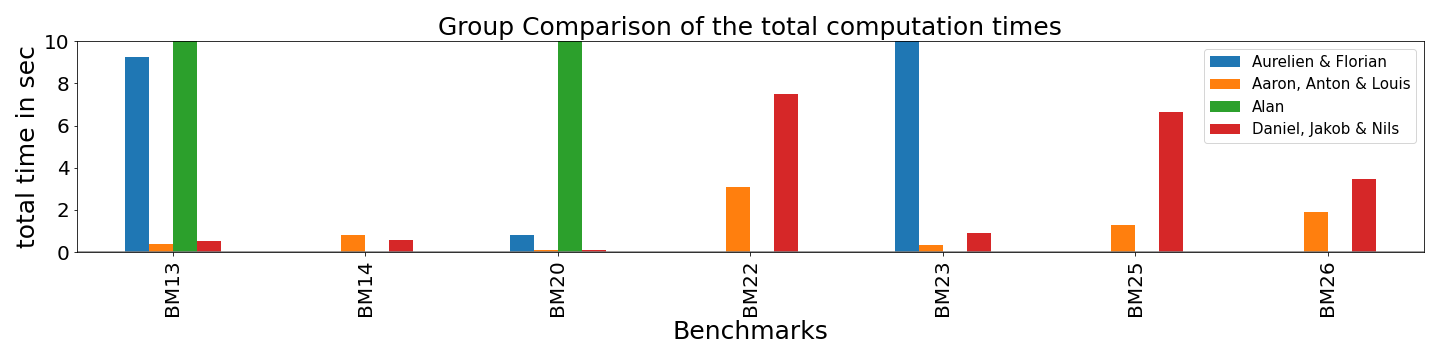
\includegraphics[scale=0.24]{images/comparison/group_comparison_total.png}
    \caption{A group comparison of the total computation time on only our large benchmarks. The y-axis is limited to 10 sec and exceeding times are cut off in this figure.}
    \label{fig:my_label}
\end{figure}
\begin{figure}
    \centering
    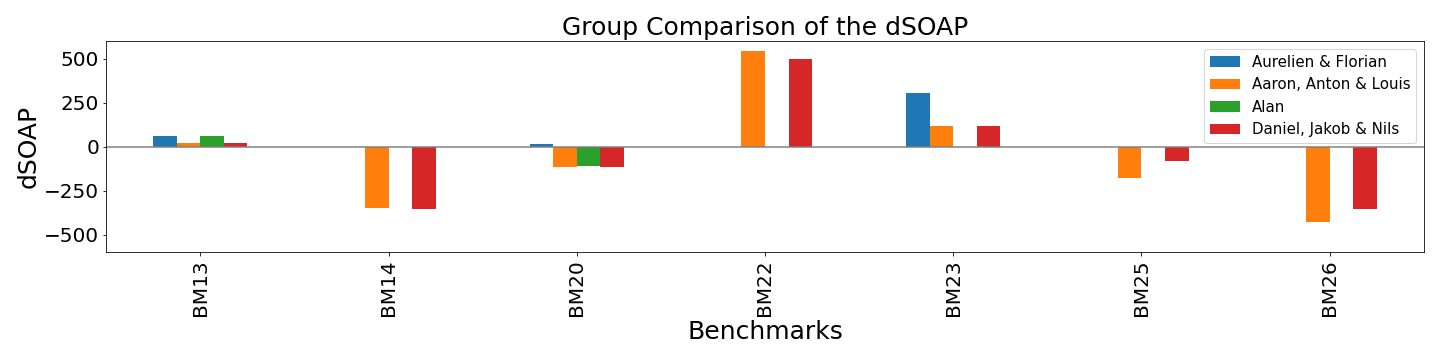
\includegraphics[scale=0.24]{images/comparison/group_comparison_SOAP.png}
    \caption{A group comparison of the dSOAP (new SOAP - original SOAP) on only our large benchmarks.}
    \label{fig:my_label}
\end{figure}

The two bar plots above allow us to gain some insight on time performance and optimality of the approaches among all groups. Unfortunately, due to problems and differences of reading the benchmark instances between the groups it as not possible to compare the results on the benchmarks of the other groups. For completeness we plotted the results of the groups on all of our benchmarks including very small ones but in order to keep the plots compact and manageable we chose to show our collection of large benchmarks once again. The results on the small benchmark instances were not very informational but it showed that Aurelien and Florian's group \cite{project2} generally had slightly shorter total computation times and Alan \cite{project3} slightly longer ones compared the the other groups. But the majority of the results were all under 0.1 seconds, so the variance alone will have a big effect.

On Fig.5 we can see four columns for each group representing the total computation time for each benchmark. The lower the column is, the shorter was the total time and if there lacks a column for a group, it means that either there was a timeout or no model found. The latter is the case for the group of Aurelien and Florian \cite{project2} and Alan \cite{project3} on Benchmark 14, 22, 25 and 26.
Also, on the large benchmark instances we can see that the total time of our group \cite{project1} and Daniel, Nils and Jacob's group \cite{project4} are mostly similar since they chose a very similar approach to ours by allowing multi-shot plan switching and a consecutive waiting step. It seems though, that on Benchmark 25 and 26 our group had faster results because the power of the deterministic waiting begins to show there.

Fig.5 shows the dSOAP of the solutions of all four groups. This plot allows us to see how optimal the models are regarding our chosen metric. While the other groups may have focused on other metrics such as the similarity to the original plans it may not be fair to compare these results directly. But a negative dSOAP indicates that path lengths have been reduced which implies that methods such as plan switching must have been used.
The plot Fig.5 quickly reveals that Aurelien and Florian's group \cite{project2} did not allow any plan switching due to the solely positive dSOAP values on the plot. On the other hand, it shows that the remaining groups all had the ability to reduce plan lengths.

\section{Conclusion}
To compare the different methods we looked at running time and the difference in sum of all positions before and after merging (dSOAP).
By choosing incremental methods over one-shot approaches we can significantly shorten the running time of the final algorithm. One disadvantage of this approach is that the program will not always be able to find the optimal solution i.e. the solution with the fewest time steps.\\
In general, we observe a trade-off between optimality and time performance. However, as the original plans already represent valid paths it can be argued that, as long as all collisions are resolved, optimizing time performance is more important than finding the shortest possible consistent plan.
Thus we prioritized improving time performance when evaluating our results.\\
It is important to note that only human made instances were used for evaluating the different approaches. We must expect real warehouse scenarios to contain more randomness as well as patterns that deterministic waiting might not be able to resolve at this stage. Even though deterministic waiting proved to be more optimal on the testing instances, we can assume that incremental waiting will perform better when dealing with new instances as the one-model approach of deterministic waiting must include a rule for every case that could come up.
Without excessive testing on more instances this can not be guaranteed.\\
Again, sequential application of the two waiting methods can be considered as deterministic waiting reliably removes collisions between many robots which are hard to resolve for \emph{Incremental Non-Deterministic Waiting}. However, right now this sequential method does not give consistent results on all benchmarks. 
This is why we decided to only use deterministic waiting if it is necessary for time performance. \\
After evaluating the effect of different features of the benchmark instances on running time we decided to base our selection of the waiting script on the number N of robots that are involved in at least one collision. If N is greater or equals to 8 we choose deterministic waiting over incremental waiting. This is based on the comparison of performance on benchmarks with different properties.
Furthermore, we decided to always try \emph{Minimal Deterministic Waiting} first as it was sufficient on many instances and only applying \emph{Comprehensive Deterministic Waiting} if the first shot does not return consistent results.
This simple algorithm for selecting the best approach can only be seen as a placeholder.\\
Taking a more in-depth look at metrics for selecting the best sequence of algorithms is interesting but beyond the scope of this paper. 
Other possibilities include omitting \emph{Preventive Plan Switching} and simply resolving new edge collisions that occur after deterministic waiting by using the naive plan switching approach.\\
When comparing our results with those of other groups we clearly observe that allowing plan switching is a massive advantage on large instances with many edge collisions. Groups that used plan switching were also able to remove more steps from the original paths. Comparing our results with the results of the other group that used plan switching we can observe the faster time performance that comes with deterministic waiting.\\
This lets us draw the following conclusions.
First, if the problem domain allows it, plan switching is a powerful tool for plan merging that drastically reduces the size of the input and can be used as a preprocessing step to transform a complicated case into a simple instance that can be solved systematically. However, it is important to understand that freely reassigning the goals is actually not possible in many real world scenarios.
\\
Additionally, repeatedly optimizing heuristics can help significantly improve time performance when generating waiting and switching positions. If time performance is more important than optimality, which we argue is the case for plan merging, greedy incremental approaches can be a valid design pattern for incremental solving.\\
Finally, on initial plans that do not include edge collision-like intersections plan merging can be solved using only waiting with a deterministic one-model approach. In general it has proved insightful to view plan merging as a problem that can be solved sequentially. Dividing the problem into smaller sub-problems proved to be central for achieving good time performance.


\newpage
\begin{thebibliography}{8}
\bibitem{amazon}
(2019). What robots do (and don’t do) at Amazon fulfilment centres.\\
https://www.aboutamazon.co.uk/news/operations/what-robots-do-and-dont-do-at-amazon-fulfilment-centres\\
\bibitem{clingo}
M. Gebser, R. Kaminski, B. Kaufmann, M. Ostrowski, T. Schaub, S. Thiele. (2010). A User’s Guide to gringo, clasp, clingo, and iclingo.\\ http://wp.doc.ic.ac.uk/arusso/wp-content/uploads/sites/47/2015/01/clingo\_guide.pdf\\
\bibitem{asprilo}
P. Obermeier and T. Otto. (2018) Asprilo.\\
https://asprilo.github.io\\
\bibitem{api}
Potassco. (n.d.). clingo API documentation.\\
https://potassco.org/clingo/python-api/5.4/\\
\bibitem{project1}
A. Bishop, A. Rabe, L. Donath. (2022). Plan Merging Project\\ https://github.com/warpaint97/plan-merging-project\\
\bibitem{project2}
A. Simon, F. Franz. (2022). KRR Project - Plan merging\\
https://github.com/Owrel/Project-KRR\\
\bibitem{project3}
A. Romer. (2022). KRR Project\\
https://github.com/AlanRomer/KRR-Projekt\\
\bibitem{project4}
D. Schreitter Ritter von Schwarzenfeld, J. Westphal and N. Bröcker. (2022). Asprilo-Project-DJN\\
https://gitup.uni-potsdam.de/nbroecker/asprilo-project-djn\\
\end{thebibliography}
\end{document}
